\section{Dynamic Programming}

\subsection{Exercise 4.1}
\subsubsection{Q}
In Example 4.1, if $\pi$ is the equiprobable random policy, what is $q_\pi(11, \mathnormal{down})$? What is $q_\pi(7, \mathnormal{down})$? 
\subsubsection{A}
The Bellman equation for $q(s,a)$ is:
\begin{equation}
q_\pi(s,a) = \sum_{s',r} p(s', r | s, a) \left[r + \gamma \sum_{a'} \pi(a' | s') q_\pi(s', a')\right]
\end{equation}

For the state-action pairs posed in the question, the Bellman equation becomes:
\begin{align}
q_\pi(11, \mathnormal{down}) &= -1 \\
q_\pi(7, \mathnormal{down}) &= -1 + -14 \\
&= -15 \\
\end{align}

as $\gamma = 1$ because MDP is undiscounted.

\subsection{Exercise 4.2}
\subsubsection{Q}
In Example 4.1, suppose a new state 15 is added to the gridworld just below state 13, and its actions, \textit{left, up, right, and down}, take the agent to states 12, 13, 14, and 15, respectively. Assume that the transitions from the original states are unchanged. What, then, is $v_pi(15)$ for the equiprobable random policy? Now suppose the dynamics of state 13 are also changed, such that action $\mathnormal{down}$ from state 13 takes the agent to the new state 15. What is $v_\pi(15)$ for the equiprobable random policy in this case?
\subsubsection{A}
\begin{align}
v_\pi(15) &= 0.25 \left[(-1 + -20) + (-1 + -22) + (-1 + -14) + (-1 + v_\pi(15)) \right] \\
&= 0.25 \left[(-60 + v_\pi(15)) \right] \\
&= -15 + 0.25 \left[v_\pi(15) \right] \\
\end{align}

and we know $v_\pi(15) == v_\pi(13) == -20$ as the state transitions and value functions at next state are identical. Therefore we get:
\begin{align}
v_\pi(15) &= -15 + 0.25 \left[-20\right] \\
&= -20 \\
\end{align}

If the dynamics are changed such one can transition from state 13 into 15, the characteristic of the MDP are unchanged. Moving into state 15, which has the same value as state 13 and the same subsequent dynamics, is identical to returning back to state 13 - as was the case previously. The value function is therefore unchanged and $v_\pi(15) = -20$

\subsection{Exercise 4.3}
\subsubsection{Q}
What are the equations analogous to (4.3), (4.4), and (4.5), but for action-value functions instead of state-value functions?
\subsubsection{A}
\begin{align}
q_\pi(s) &= \mathbb{E}_\pi \left[R_{t+1} + \gamma q_\pi(S_{t+1}, A_{t+1} | S_t = s, A_t = a)\right]v_\pi(s) \\
q_\pi(s,a) &= \sum_{s',r} p(s', r | s, a) \left[r + \gamma \sum_{a'} \pi(a' | s') q_\pi(s', a')\right] \\
q_{k+1}(s,a) &= \sum_{s',r} p(s', r | s, a) \left[r + \gamma \sum_{a'} \pi(a' | s') q_k(s', a')\right] \\
\end{align}

\subsection{Exercise 4.4}
\subsubsection{Q}
The policy iteration algorithm on page 80 has a subtle bug in that it may never terminate if the policy continually switches between two or more policies that are equally good. This is okay for pedagogy, but not for actual use. Modify the pseudocode so that convergence is guaranteed.
\subsubsection{A}
When taking the argmax over $a$ in the policy improvement step of the algorithm, it's possible that we continue to flip backward and forward between two actions that are both optimal forever. At the moment, a tie is broken by randomly selecting between the value maximising actions. We could instead always select the first action to result from the argmax, this way we would ensure that the same optimal action is picked during iteration, switching the \textit{policy-stable} boolean to true, and ensuring convergence.

\subsection{Exercise 4.5}
\subsubsection{Q}
How would policy iteration be defined for action values? Give a complete algorithm for computing $q_*$, analogous to that on page 80 for computing $v_*$. Please pay special attention to this exercise, because the ideas involved will be used throughout the rest of the book.
\subsubsection{A}
\begin{enumerate}
	\item \textbf{Initialization}: $q(s,a)$ and $\pi(s)$ initialised arbitrarily as before
	\item \textbf{Policy Evaluation}: Loop for each state-action pair $(s,a)$, $s \in \mathcal{S}, a \in \mathcal{A}$:\\
	\begin{equation}
	\begin{aligned}
		q \leftarrow Q(s,a) \\
		Q(s,a) \leftarrow \sum_{s',r} p(s', r | s, a) \left[r + \gamma \sum_{a'} \pi(a' | s') Q(s', a')\right] \\
		\delta \leftarrow max(\delta, |q - Q(s,a)|)
	\end{aligned}
	\end{equation}
	\item \textbf{Policy Improvement}: \\
	\begin{equation}
	\begin{aligned}
		\text{policy-stable} \leftarrow True \\
		\text{Loop for each state-action pair (s,a), s $\in \mathcal{S}, a \in \mathcal{A}$}:\\
		old-action \leftarrow \pi(s)\\
		\pi(s) \leftarrow \argmax_a \sum_{s',r} p(s', r | s, a) \left[r + \gamma \sum_{a'} \pi(a' | s') q_\pi(s', a')\right] \\
		\text{if old-action} \neq \pi(s), \text{then policy-stable} \leftarrow False \\
		\text{If policy-stable, then stop and return Q $\approx q_* and \pi \approx \pi_*$; else return to 2.} \\
	\end{aligned}
	\end{equation}
\end{enumerate}

\subsection{Exercise 4.6}
\subsubsection{Q}
Suppose you are restricted to considering only policies that are $\epsilon$-soft, meaning that the probability of selecting each action in each state, $s$, is at least $\epsilon /|\mathcal{A}(s)|$. Describe qualitatively the changes that would be required in each of the steps 3, 2, and 1, in that order, of the policy iteration algorithm for $v_*$ on page 80.
\subsubsection{A}
During the policy improvement step (3), instead of the argmax creating a deterministic action in a state, we would update the policy such that each action $a \in \mathcal{A}$ would receive probability p(a) = $\epsilon /|\mathcal{A}(s)|$, then the max action would receive probability $1 - \epsilon + \epsilon /|\mathcal{A}(s)|$. The output policy is therefore stochastic, not deterministic. During the policy evaluation step (2), instead of looping over the states only, we would loop over all states and actions, weighting the value of each state-action by the probability of the action being selecting according to our $\epsilon$-soft policy. In step one, the policy would need to be initialised with an arbitrary distribution over the action space in each state.

\subsection{Exercise 4.7}
\subsubsection{Q}
Write a program for policy iteration and re-solve Jack’s car rental problem with the following changes. One of Jack’s employees at the first location rides a bus home each night and lives near the second location. She is happy to shuttle one car to the second location for free. Each additional car still costs \$2, as do all cars moved in the other direction. In addition, Jack has limited parking space at each location. If more than 10 cars are kept overnight at a location (after any moving of cars), then an additional cost of \$4 must be incurred to use a second parking lot (independent of how many cars are kept there). These sorts of non-linearities and arbitrary dynamics often occur in real problems and cannot easily be handled by optimization methods other than dynamic programming. To check your program, first replicate the results given for the original problem.
\subsubsection{A}
\ProgrammingExercise

\subsection{Exercise 4.8}
\subsubsection{Q} Why does the optimal policy for the gambler’s problem have such a curious form? In particular, for capital of 50 it bets it all on one flip, but for capital of 51 it does not. Why is this a good policy?
\subsubsection{A}
When the coin is bias against us it makes sense to minimise the number of flips we make as, in the limit, we cannot win. Consequently, we can win with probability 0.4 is we stake our full capital at 50. All other bets besides 50 are designed to get us back to 50 if we lose, or up to 50 if we win, from where we take our 40\% chance. For example, when our capital is 55, we stake 5, knowing that we are likely to fall back to 50 where we will go for the win.

\subsection{Exercise 4.9}
\subsubsection{Q} Implement value iteration for the gambler’s problem and solve it for $p_h$ = 0.25 and $p_h$ = 0.55. In programming, you may find it convenient to introduce two dummy states corresponding to termination with capital of 0 and 100, giving them values of 0 and 1 respectively. Show your results graphically, as in Figure 4.3. Are your results stable as $\theta \rightarrow 0$?
\subsubsection{A}
\ProgrammingExercise

\begin{figure}[h!]
	\centering
	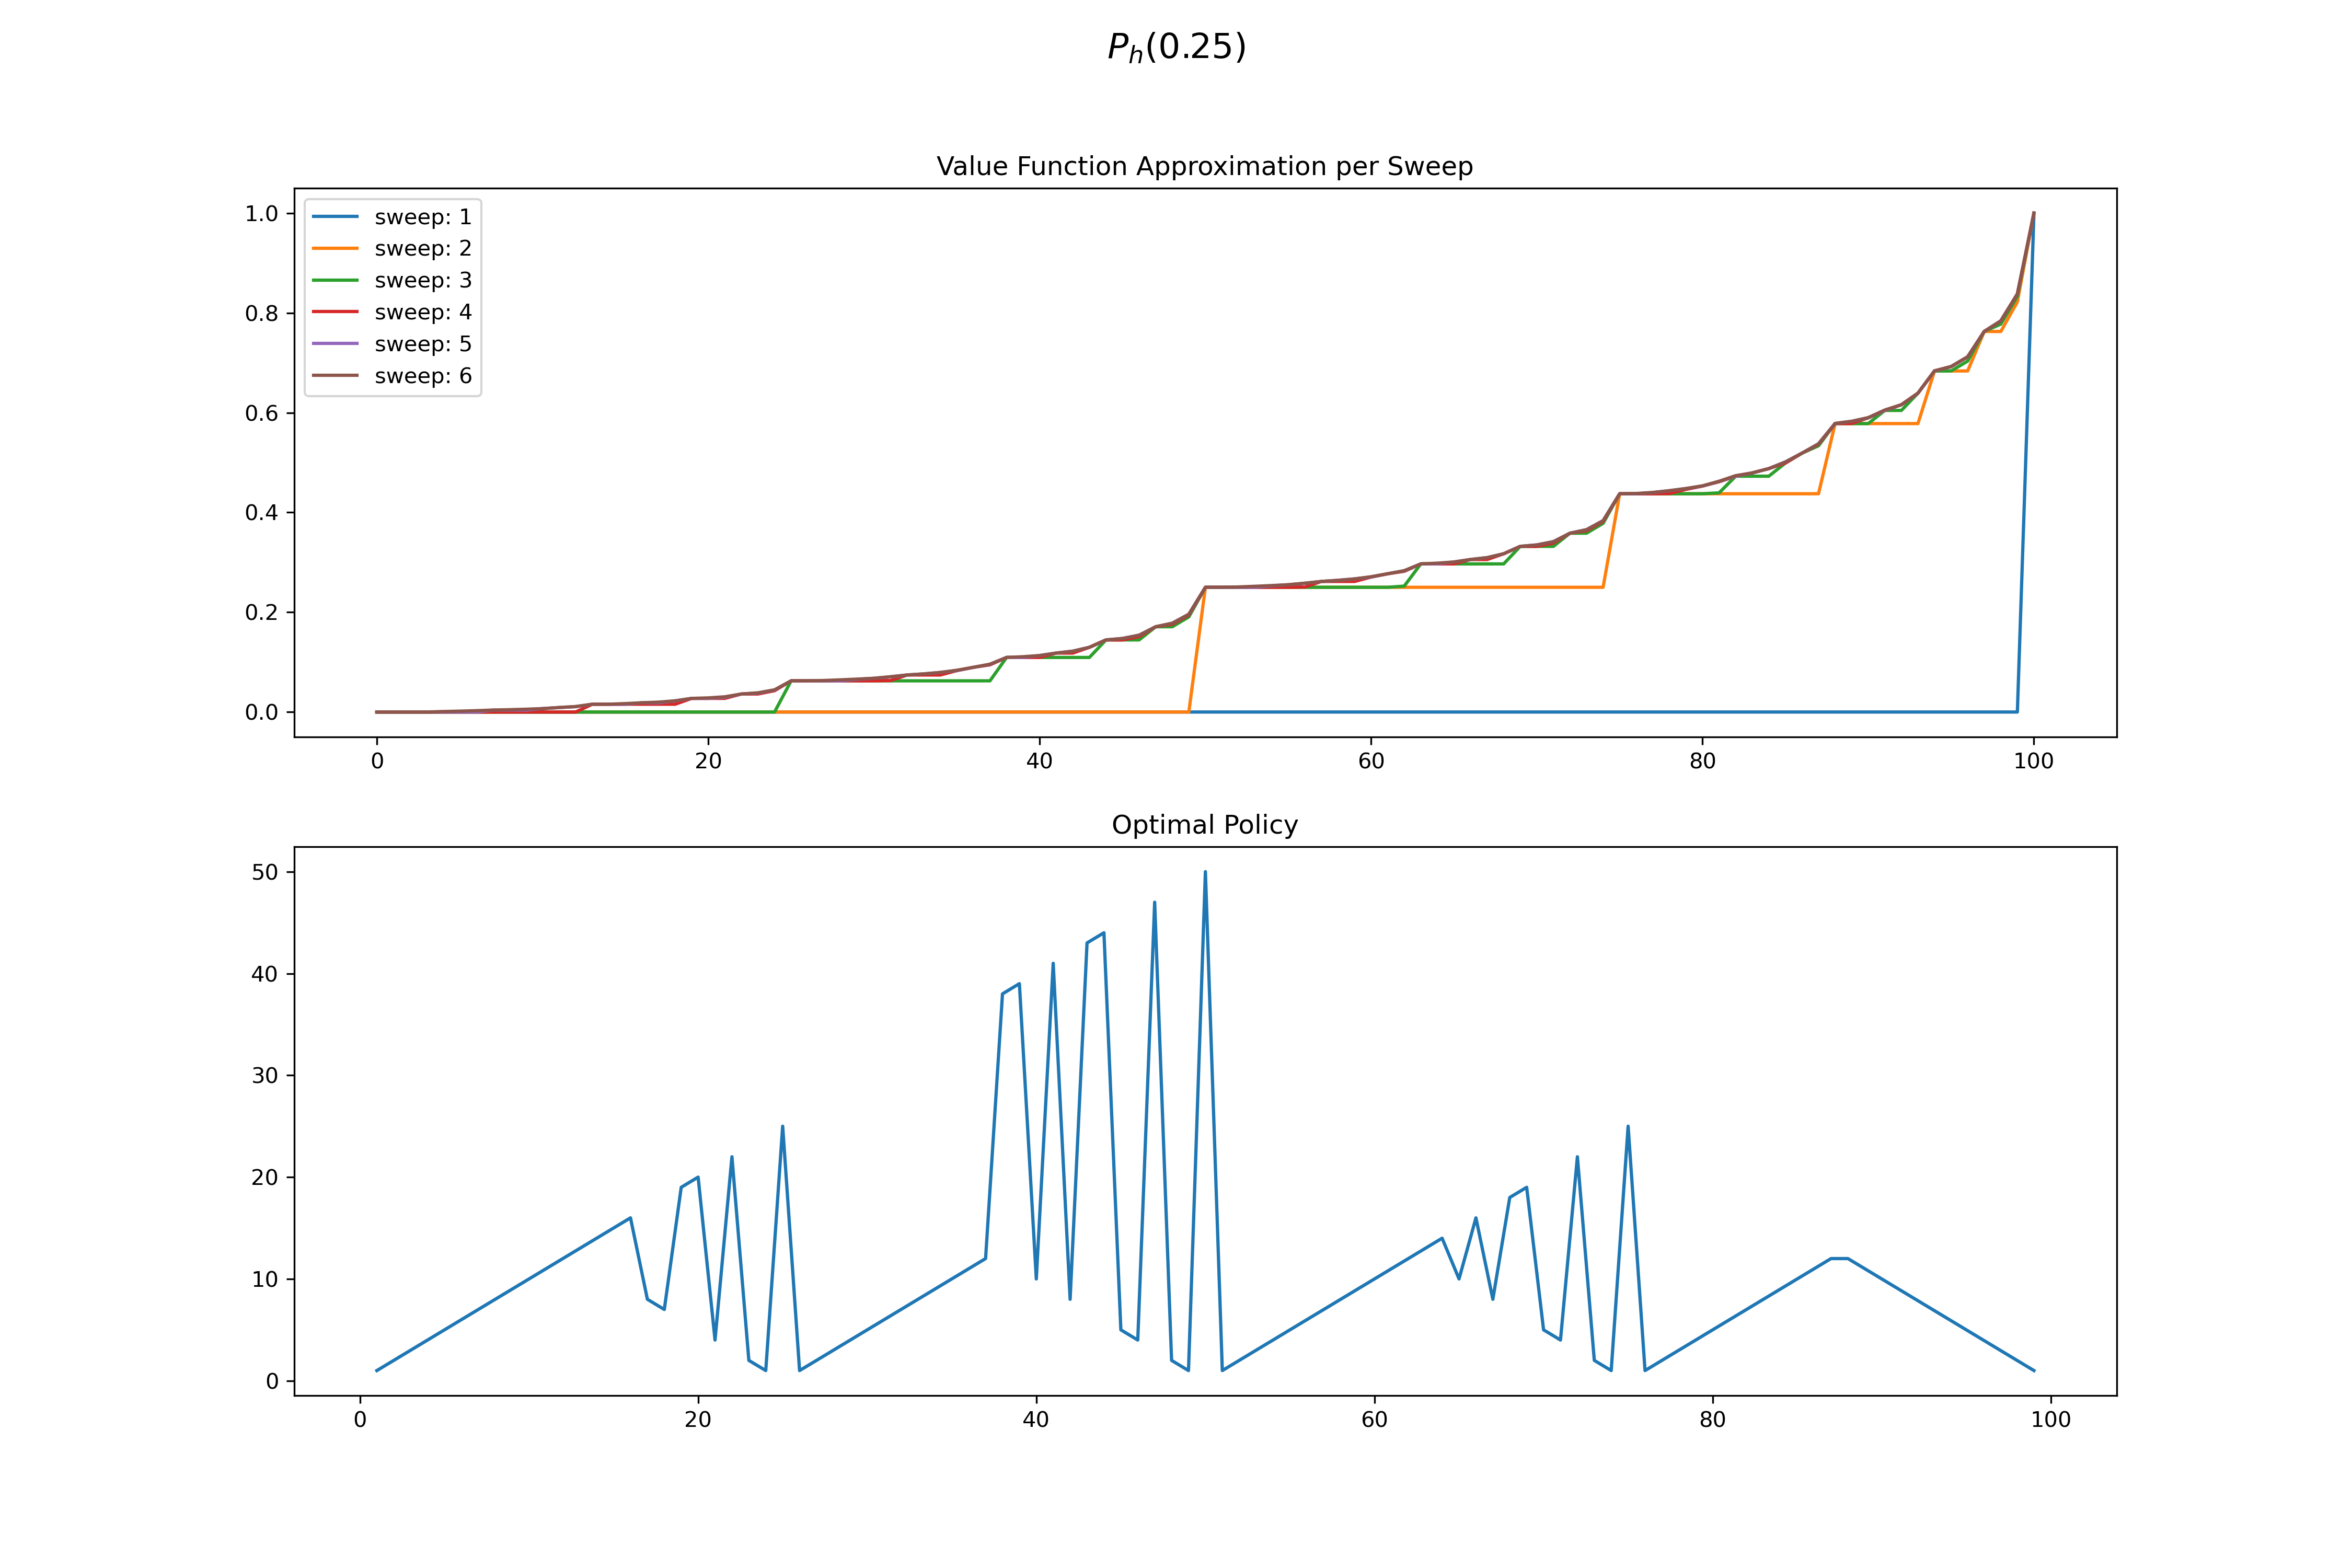
\includegraphics[width=\textwidth]{/ex4.9a}
	\label{fig:4.9a}
\end{figure}

\begin{figure}[h!]
	\centering
	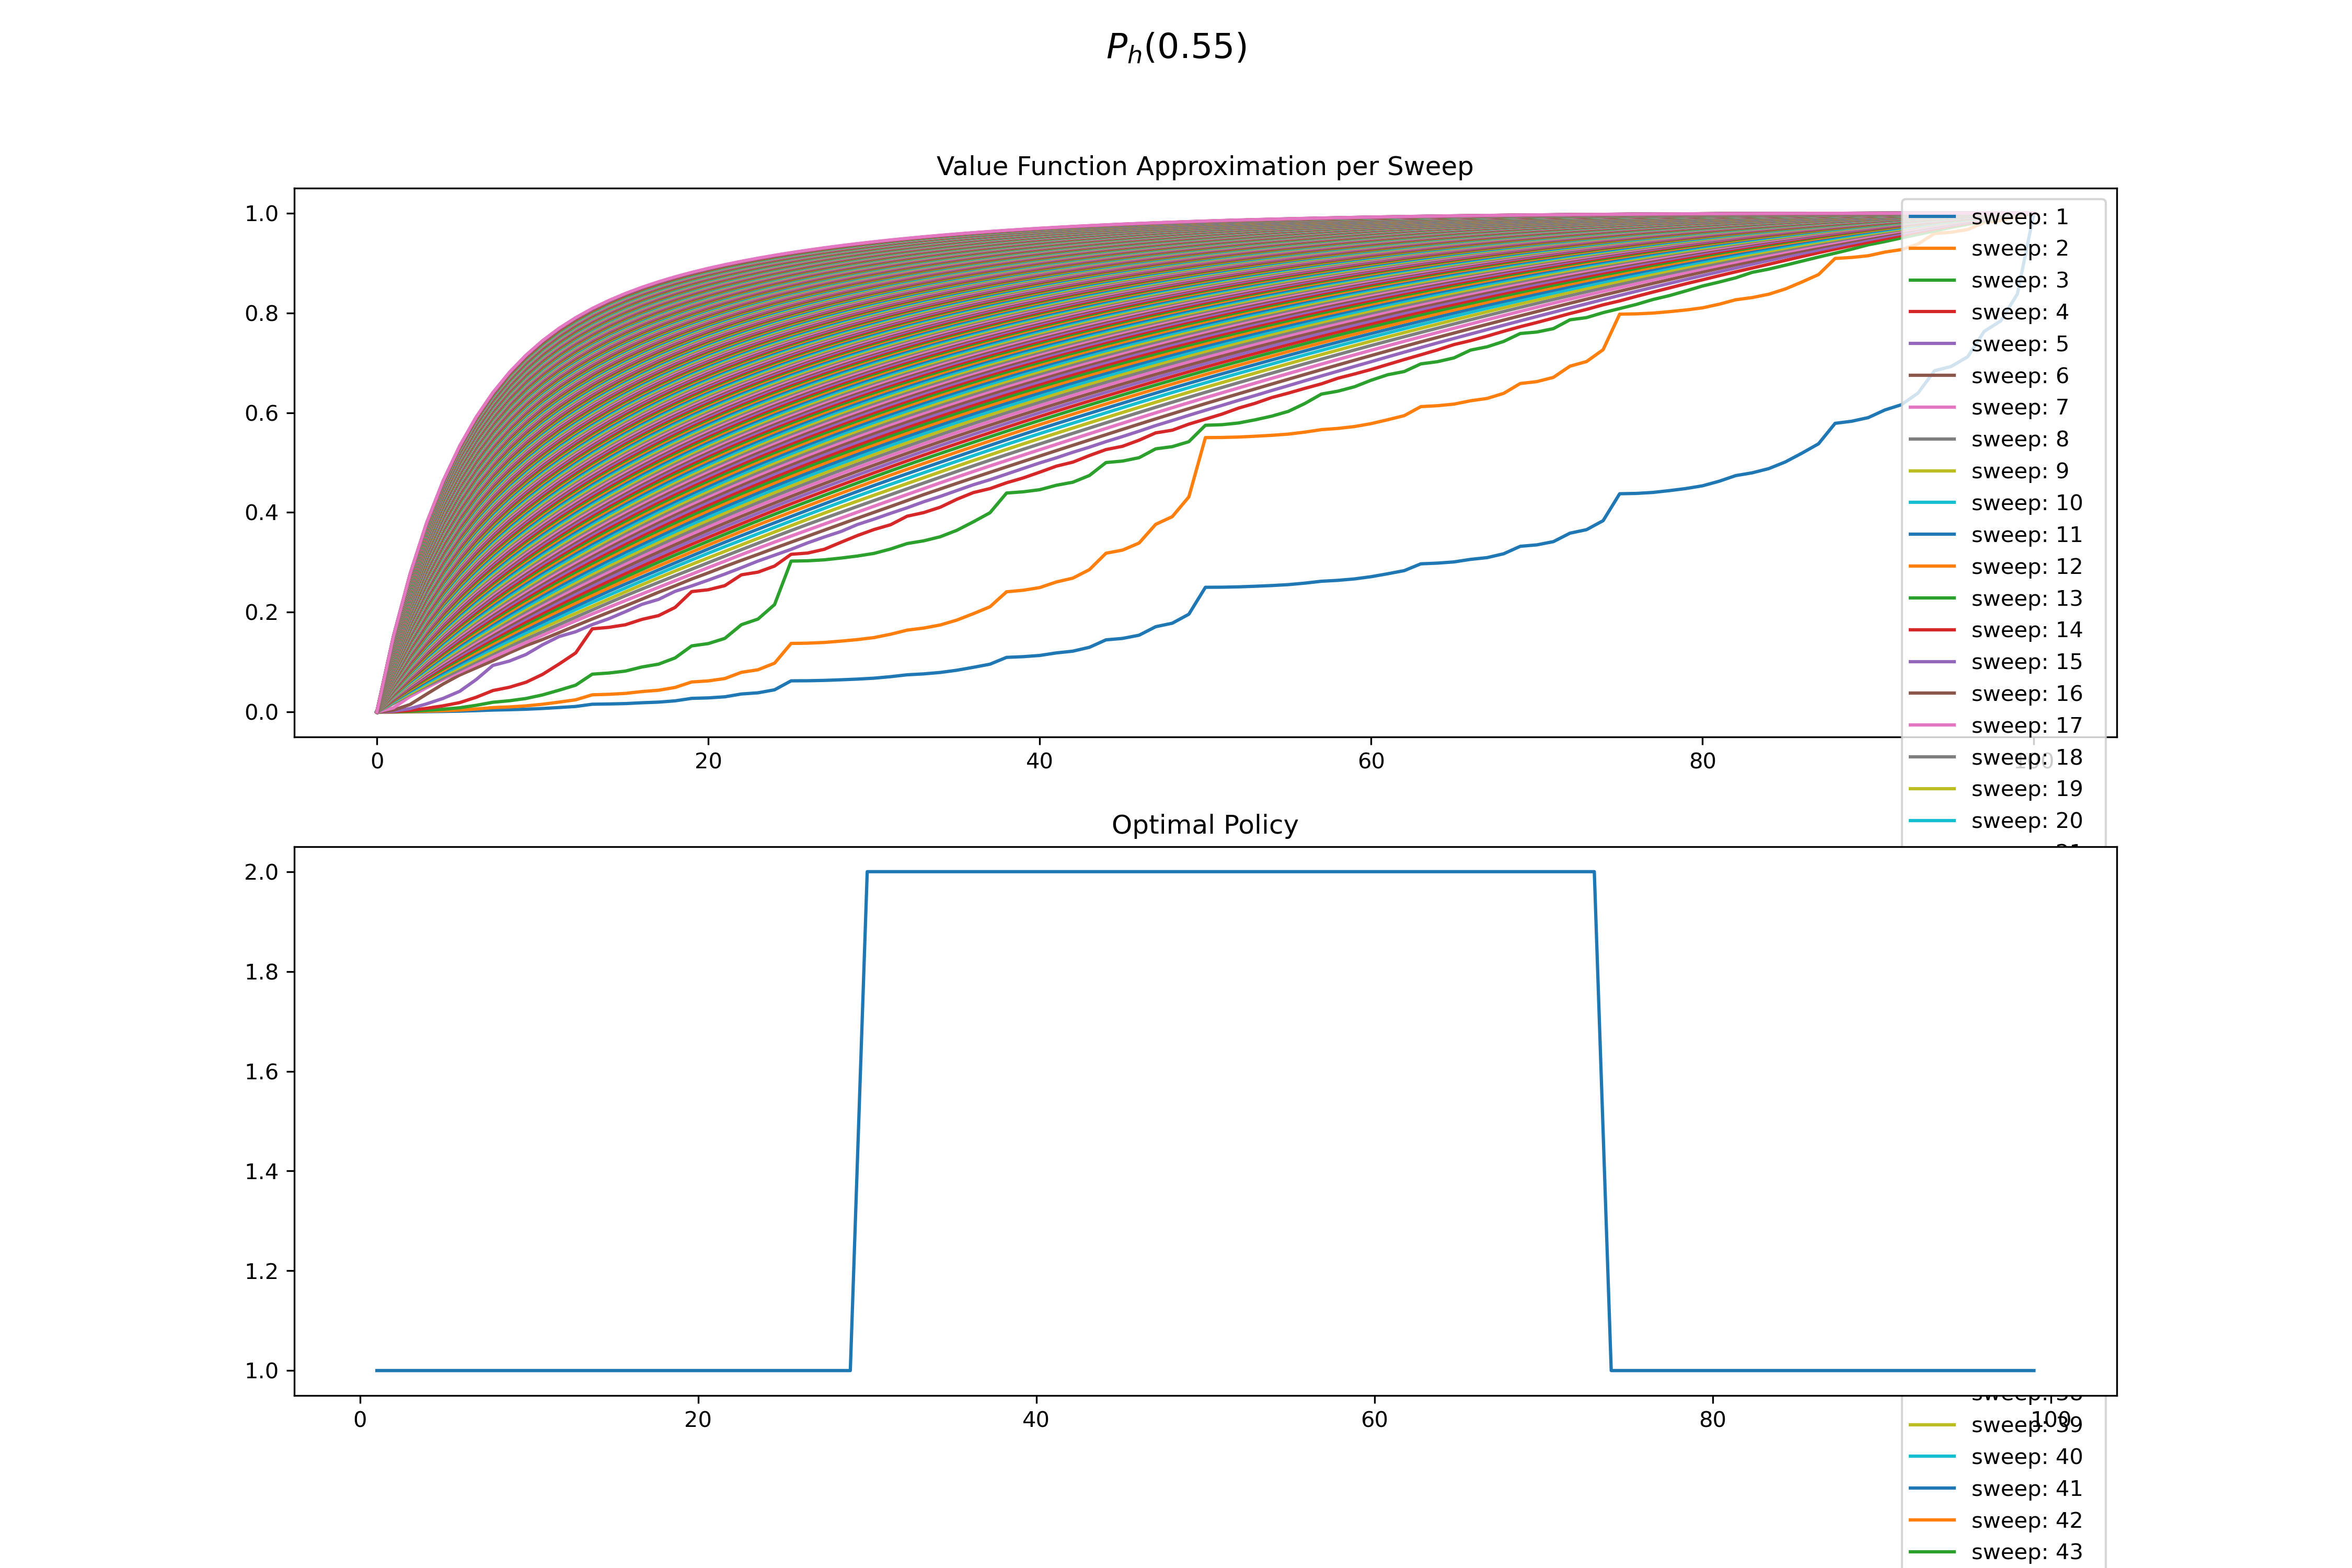
\includegraphics[width=\textwidth]{/ex4.9b}
	\label{fig:4.9b}
\end{figure}

\subsection{Exercise 4.10}
\subsubsection{Q} What is the analog of the value iteration update (4.10) for action values, $q_{k+1}(s, a)$?
\subsubsection{A}
\begin{equation}
v_{k+1}(s) =  \sum_{s',r} p(s', r |s, a)\left[r + \gamma \argmax_{a'} q_k(s', a')\right]
\end{equation}
